\subsubsection{Diffusjon}
Et n-type stoff ved siden av et p-type stoff, fører til diffusjon.
De svakt bundede elektronene i n-type swoopper over
til hullene i p-type.
Dette kalles \emph{diffusjon}.
\\
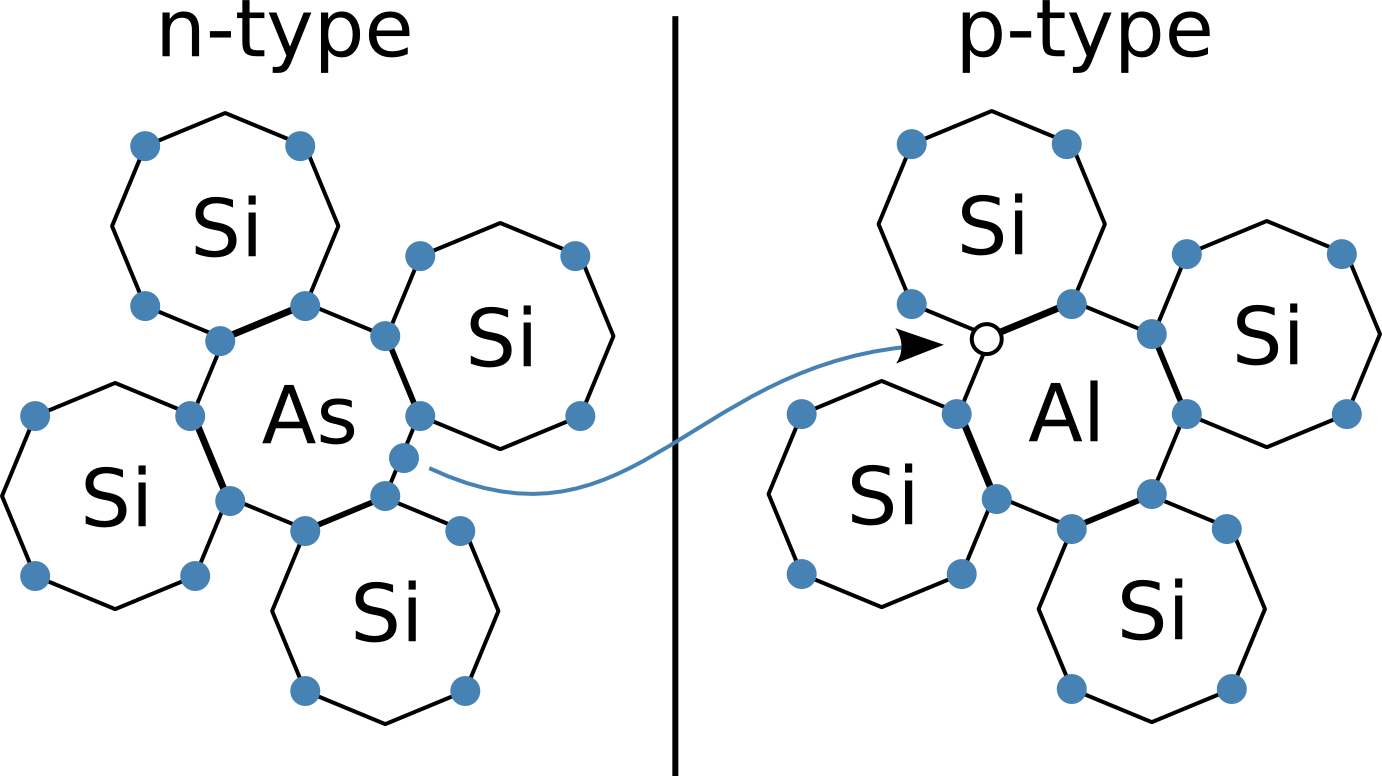
\includegraphics[width=\textwidth]{./img/krystall-pn}

\subsubsection{Sperresjikt}
Hvis man setter sammen n-type og p-type materialer,
vil det ved diffusjon trekkes elektroner
fra n-type over til p-type.
\\\\
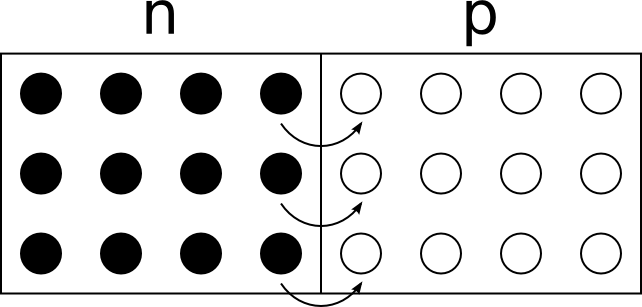
\includegraphics[width=0.67\textwidth]{./img/pn-junction}
\\\\
Elektronene \emph{rekombinerer} med hull på den andre siden,
og etterlater seg hull der de kom fra.
\\\\
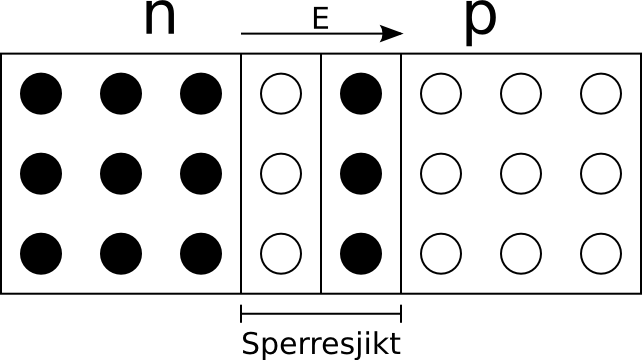
\includegraphics[width=0.67\textwidth]{./img/pn-sperresjikt}
\\
Det skapes et sperresjikt (depletion layer) mellom materialene.
Dette sjiktet fungerer som en isolator og stopper videre overføring.
\\
Sperresjiktet har en potensialbarriere på 0.3 - 0.7 Volt,
avhengig av materiale.

\subsubsection{Forward bias}
Når man påfører en spenning til en PN-Junction
vil elektroner bevege seg mot positiv terminal.
\\
Elektronene på p-side vil forlate sin posisjon og gå mot positiv.
Elektroner på n-side vil bevege seg mot positiv
og fylle igjen hullene i n-side på veien.
\\
Spenningsjiktet er nå brutt ned og strøm kan gå gjennom.
\\\\
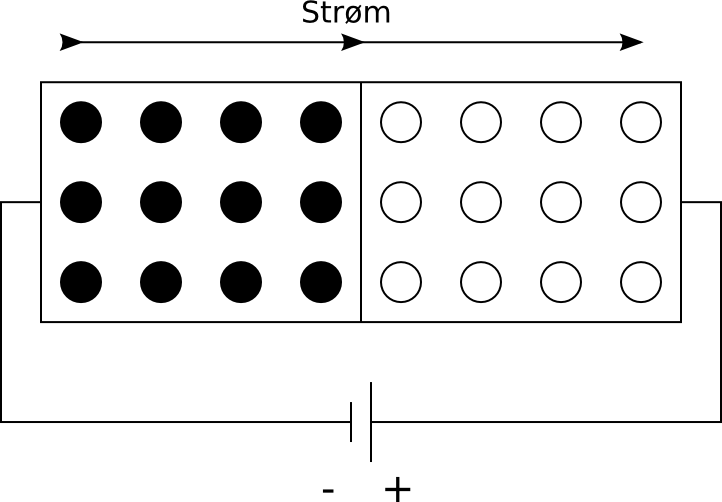
\includegraphics[width=0.67\textwidth]{./img/pn-forward}

\subsubsection{Reverse bias}
Reverserer man spenningskilden går elektronene andre vei.
\\
Elektronene på n-side vil gå mot positiv terminal
og etterlate seg hull på sin egen side.\\
Elektroner fra negativ terminal frastøter elektroner på p-side.
Disse beveger seg \emph{fra} negativ,
intill de møter den positive barrieren på n-side.
\\\\
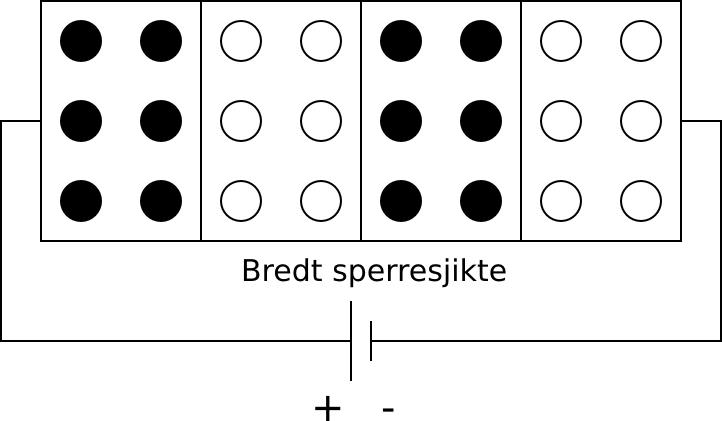
\includegraphics[width=0.67\textwidth]{./img/pn-reverse}
